\chapter{\tenKL}
\label{Chapter3}

% Dẫn nhập: mô tả chi tiết phương pháp thực hiện và giải pháp đề xuất trên mô hình, bo mạch, giao diện web, và hệ thống back-end
Chương \ref{Chapter3} mô tả chi tiết phương pháp thực hiện và giải pháp đề xuất trên mô hình hệ thống \acrshort{iot}. Các mô tả này bao gồm mô hình, bo mạch, giao diện web, và hệ thống back-end.

\section{Mô hình hệ thống IoT}

% Tổng quan về mô hình: phần cứng, máy chủ ảo.
Mô hình hệ thống \acrshort{iot} được đề xuất (minh họa như hình \ref{fig:IoT-Model-Overral}), được triển khai dựa trên sự kết hợp của bo mạch, hệ thống back-end, giao diện web, và giao thức kết nối giữa chúng. Dựa trên các thành phần này, mô hình \acrshort{iot} 4 lớp (được đề cập ở mục \ref{Model-Diagram-IoT-System}) sẽ được áp dụng. Trên mô hình này, bo mạch của \acrshort{ptn} DESLab và \acrshort{vps} của các quản trị viên \acrshort{vnpt} là hai thành phần chủ đạo.

Trên bo mạch, bo mạch được thiết kế dựa trên kết nối của các \acrshort{mcu} STM32 và ESP32. Trong đó, \acrshort{mcu} STM32 là thiết bị giao tiếp vạn vật (things) và thuộc sensing layer. Tiếp theo, \acrshort{mcu} ESP32 là \acrshort{iot} gateway định tuyến các luồng dữ liệu trong giao tiếp sensing-network layer và thuộc lớp network layer.

Trên \acrshort{vps}, hệ thống \acrshort{iot} triển khai hệ thống back-end và Nginx web server. Cụ thể, hệ thống back-end bao gồm \acrshort{mqtt} Broker, EggJS \acrshort{api} server, và MongoDB database. Cuối cùng, Nginx web server cung cấp giao diện người dùng và giao diện người dùng được phát triển trên nền tảng ReactJS và giải pháp Ant Design Pro.

Trên hệ thống \acrshort{iot}, hệ thống có 3 kỹ thuật xử lý dữ liệu. Đó là giao thức frame, mật mã hóa nhẹ ChaCha20-Poly1305, và đồng bộ. Trong đó, giao thức frame được triển khai trên thiết bị STM32, ESP32 gateway, và \acrshort{api} server. Tiếp theo, mật mã hóa ChaCha20-Poly1305 được sử dụng trên ESP32 gateway và \acrshort{api} server. Cuối cùng, cơ chế đồng bộ được triển khai trên \acrshort{api} server, giao diện web, và thiết bị STM32.

Về các giao thức truyền, hệ thống sử dụng giao thức có dây \acrfull{uart}; các giao thức không dây: \acrshort{mqtt}, \acrfull{https}, và Websocket; và \acrfull{vlan}. Trong đó, \acrshort{uart} được sử dụng trong giao tiếp gateway-device; \acrshort{mqtt} được sử dụng trong giao tiếp gateway-\acrshort{mqtt} Broker và \acrshort{mqtt} Broker-\acrshort{api} server; \acrshort{https} và Websocket được sử dụng trong giao tiếp \acrshort{api} server-web; và \acrshort{vlan} được sử dụng trong giao tiếp \acrshort{api}~server-database.

\begin{figure}[htp]
\centering
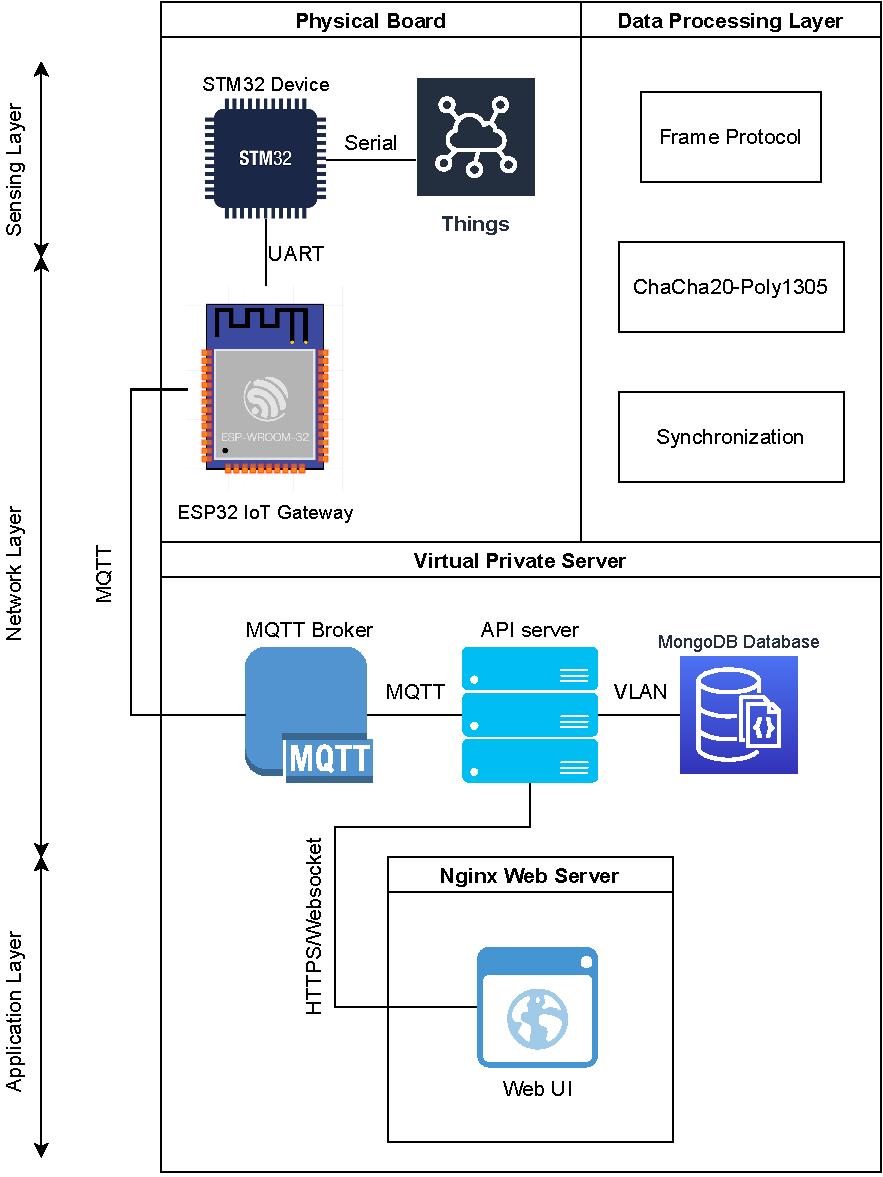
\includegraphics[width=1.0\linewidth]{images/Thesis-Page-8-IoT-Model-Overral.pdf}
\caption{Mô hình hệ thống \acrshort{iot} được đề xuất.}
\label{fig:IoT-Model-Overral}
\end{figure}

% Nội dung về bo mạch phát triển, các kỹ thuật trên bo mạch.
\section{Bo mạch phần cứng}

% Giới thiệu về bo mạch
Bo mạch phần cứng được sử dụng để xây dựng hệ thống \acrshort{iot} (minh họa ở hình \ref{fig:IoT-Dev-Board}), là bo mạch phát triển \acrshort{iot} của \acrshort{ptn} DESLab. Bo mạch này bố trí hai \acrshort{mcu} STM32F407VGT6 và ESP Wroom 32 kèm theo các ngoại vi. Các ngoại vi bao gồm led, nút nhấn, switch, màn hình OLED, và các \acrshort{gpio} của hai \acrshort{mcu}.

\begin{figure}[htp]
\centering
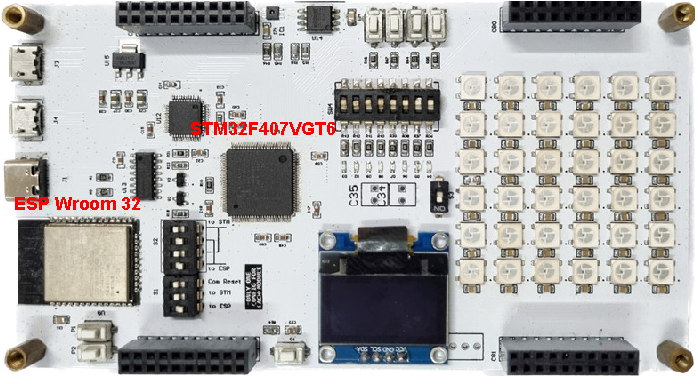
\includegraphics[width=1.0\linewidth]{images/Thesis-Page-1-Bo-mach.pdf}
\caption{Bo mạch phát triển \acrshort{iot} của \acrshort{ptn} DESLab.}
\label{fig:IoT-Dev-Board}
\end{figure}

% Chỉ trình bày chi tiết về chức năng của các MCU, ko giải thích source
\subsection{ESP32 IoT gateway}
\label{ESP32-IoT-gateway}

% Mục đích sử dụng, giới thiệu về các chức năng sẽ trình bày.
\acrshort{mcu} ESP32 được phát triển trên framework Arduino, platform PlatformIO, và ngôn ngữ C++. ESP32 được bố trí trên bo mạch phát triển và có sẵn module WiFi (Wi-Fi: 802.11 b/g/n/e/i, 2.5 GHz). Vì vậy, \acrshort{mcu} ESP32 được phát triển để được sử dụng như một \acrshort{iot} gateway. Về cơ bản, ESP32 \acrshort{iot} gateway có nhiệm vụ định tuyến các luồng dữ liệu trong giao tiếp STM32 device-\acrshort{api} server và ngược lại. Để thực hiện được công việc này, \acrshort{mcu} ESP32 phải thực hiện công việc phân giải và xử lý frame giao tiếp cũng như đệm dữ liệu (buffering data).

Về việc đệm dữ liệu, \acrshort{mcu} ESP32 sử dụng bộ đệm vòng (circular buffer) có kích thước cố định để lưu trữ tạm thời các dữ liệu nhận được. Trên bo mạch hiện tại, ESP32 có hai bộ đệm vòng để nhận dữ liệu qua giao tiếp \acrshort{uart} từ \acrshort{mcu} STM32 và qua giao tiếp \acrshort{mqtt} từ \acrshort{mqtt} Broker. Cụ thể, bộ đệm vòng UART nhận dữ liệu từ ngắt \acrshort{uart} và bộ đệm vòng \acrshort{mqtt} nhận dữ liệu từ \acrshort{mqtt} message callback. Dựa trên các buffer này, ESP32 tiến hành phân xử từng buffer (minh họa như hình \ref{fig:CBuf-Abritrating}) trong vòng lặp vô hạn của firmware. Để phân xử hợp lý cho từng bộ đệm, buffer selector được triển khai để lựa chọn buffer trong mỗi vòng lặp. Việc này giúp các buffer luôn được kiểm tra và mỗi buffer sẽ được tiến hành xý lý khi nó có dữ liệu.

\begin{figure}[htp]
\centering
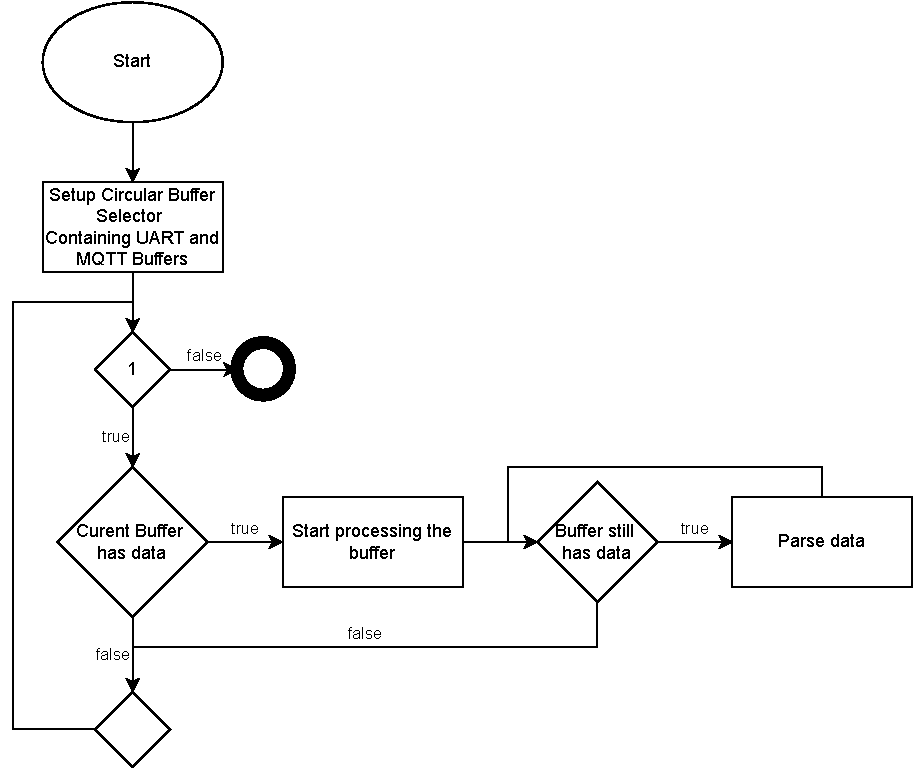
\includegraphics[width=1.0\linewidth]{images/Thesis-Page-9-CBuf-Abritrating.pdf}
\caption{Quá trình phân xử các bộ đệm vòng.}
\label{fig:CBuf-Abritrating}
\end{figure}

Về quá trình phân giải và xử lý frame, quá trình này diễn ra để xử lý dữ liệu trong bộ đệm vòng. Khi bộ đệm có dữ liệu, quá trình phân giải frame sẽ diễn ra trong một process độc lập (minh họa như hình \ref{fig:Frame-Parsing-Process}). Process này sẽ kết thúc khi frame được phân giải thành công, thất bại, hoặc timeout.

\begin{figure}[htp]
\centering
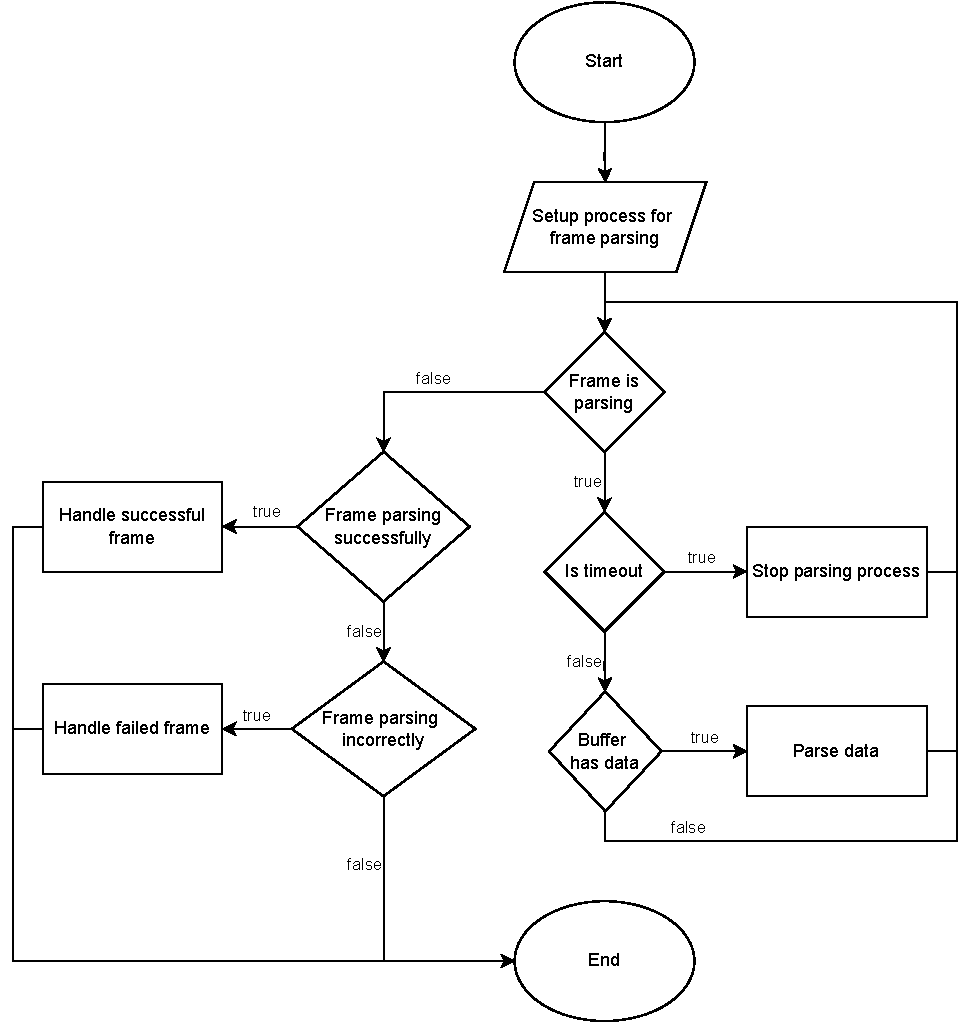
\includegraphics[width=1.0\linewidth]{images/Thesis-Page-10-Frame-Parsing-Process.pdf}
\caption{Process phân giải frame.}
\label{fig:Frame-Parsing-Process}
\end{figure}

\subsection{STM32 device}

\acrshort{mcu} STM32 được phát triển trên công cụ STM32CubeIDE và sử dụng ngôn ngữ C. STM32 được phát triển như một thiết bị vật lý trong mô hình \acrshort{iot}. Cụ thể, \acrshort{mcu} STM32 có nhiệm vụ tương tác với các cảm biến và ngoại vi cũng như đồng bộ dữ liệu với \acrshort{api} server.

STM32 thực hiện đệm dữ liệu, xử lý và phân giải frame như ESP32 gateway (được đề cập trong mục \ref{ESP32-IoT-gateway}). Ngoài ra, STM32 có thể đọc và thay đổi cơ sở dữ liệu trên \acrshort{vps} thông qua các \acrshort{api}. Các \acrshort{api} này giúp STM32 gửi yêu cầu đọc ghi dữ liệu và đồng bộ với cơ sở dữ liệu. Các \acrshort{api} này bao gồm \acrshort{api} đọc dữ liệu của \acrshort{vs}; và ghi dữ liệu \acrshort{vs} theo kiểu Integer và Float.

\section{Hệ thống back-end}

Hệ thống back-end là tập hợp những ứng dụng server chạy trên \acrshort{vps}. Những ứng dụng này bao gồm \acrshort{mqtt} Broker, \acrshort{api} server, và MongoDB database. Trên \acrshort{vps}, hệ thống back-end được triển khai bằng kỹ thuật Docker Containerizing.

\subsection{MQTT Broker}

\acrshort{mqtt} Broker, trung tâm của giao thức Publish/Subscribe \acrshort{mqtt}, là một ứng dụng server thu nhận tất cả các message từ các \acrshort{mqtt} client và định tuyến đến những subscribing client thích hợp \cite{MQTT-Broker-Def}.

Trong hệ thống \acrshort{iot} được đề xuất, \acrshort{mqtt} Broker được xây dựng trên framework NodeJS và ngôn ngữ JavaScript. Trong \acrshort{mqtt} Broker, các \acrshort{mqtt} client là \acrshort{iot} gateway và \acrshort{api} server. Hơn nữa, các dữ liệu publish/subscribe trên \acrshort{mqtt} Broker đều được mã hóa bởi thuật toán ChaCha20-Poly1305.

% Mô hình
Về tổ chức kết nối, giao thức \acrshort{mqtt} sử dụng các topic để quản lý luồng dữ liệu. Trên hệ thống \acrshort{iot}, các gateway và \acrshort{api} server sẽ được tổ chức kết nối \acrshort{mqtt} thông qua việc publish/subscribe (minh họa như hình \ref{fig:Frame-Parsing-Process-2}). Trong đó, \acrshort{api} server subscribe vào một topic và các gateway cùng gửi dữ liệu từ phần cứng vào cùng một topic đó. Trong khi, các gateway sẽ subscribe vào một topic riêng biệt và \acrshort{api} server gửi dữ liệu tới phần cứng thông qua từng topic riêng biệt đó. Các topic của gateway được phân biệt thông qua 12-byte gateway ID.

\begin{figure}[htp]
\centering
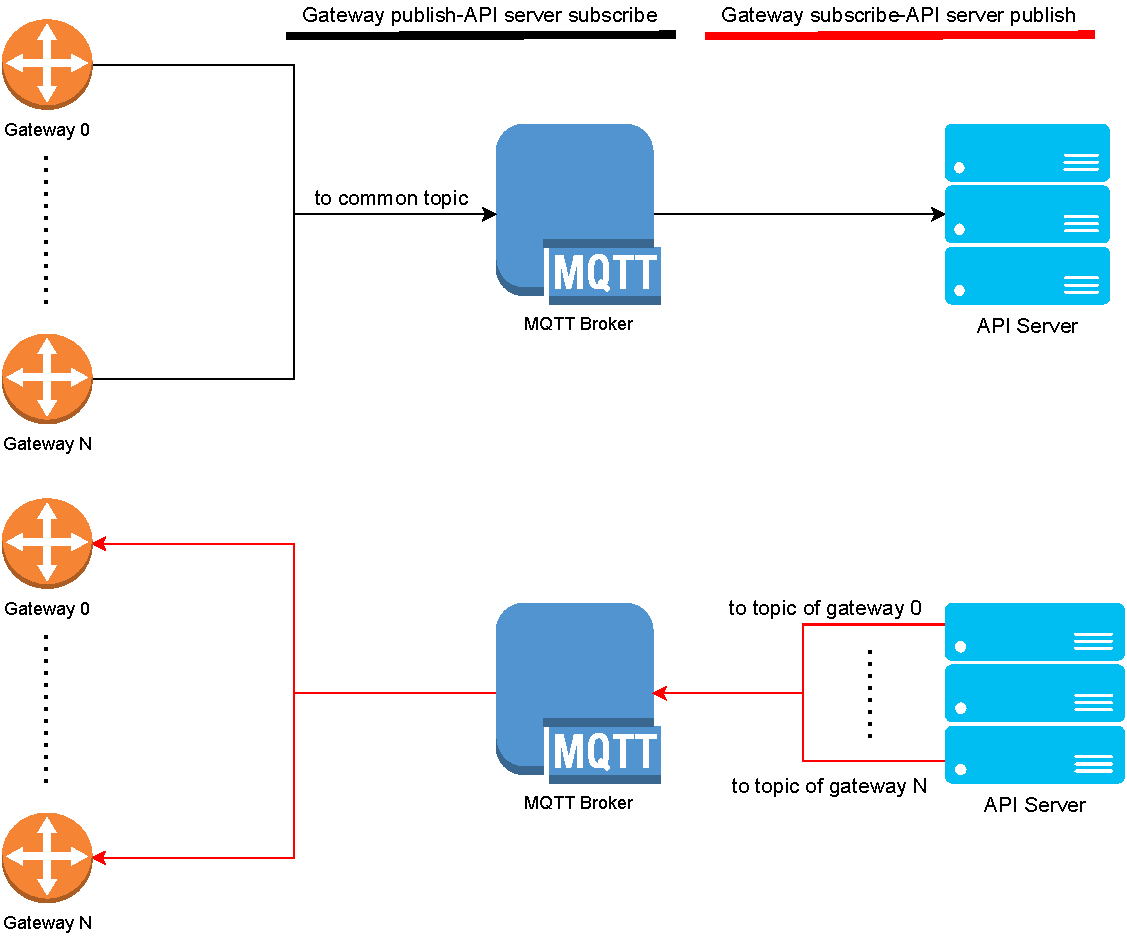
\includegraphics[width=1.0\linewidth]{images/Thesis-Page-11-MQTT-Connect-Establish.pdf}
\caption{Mô hình Publish/Subscribe MQTT trên hệ thống IoT.}
\label{fig:Frame-Parsing-Process-2}
\end{figure}

% Tổng quan, kết nối với thiết bị, kết nối với CSDL, và web.
\subsection{API Server}

\acrshort{api} server, trung tâm của hệ thống \acrshort{iot}, là ứng dụng server được xây dựng trên nền tảng EggJS, môi trường NodeJS, và ngôn ngữ JavaScript. Trên hệ thống, \acrshort{api} server có nhiệm vụ thu nhận và xử lý dữ liệu cũng như cung cấp dịch vụ truy xuất database cho phần cứng và giao diện web. Cụ thể, \acrshort{api} server thu nhận và xử lý dữ liệu phần cứng thông qua giao thức \acrshort{mqtt} và dữ liệu từ giao diện web thông qua giao thức \acrshort{https}. Cuối cùng, \acrshort{api} server là một điểm kết nối với database và cung cấp các dịch vụ truy xuất và sự kiện từ database.

\subsubsection{Giao tiếp với phần cứng}

\acrshort{api} server giao tiếp với phần cứng thông qua kết nối \acrshort{mqtt} Broker và đóng vai trò là một \acrshort{mqtt} client. Trên giao tiếp này, giao thức frame (được đề cập ở mục \ref{Frame-Protocol-subsec}) được sử dụng để truyền và nhận dữ liệu từ phần cứng.
% Các dữ liệu trao đổi với phần cứng.
Cấu trúc gói dữ liệu trên frame giao tiếp với phần cứng (minh họa như hình \ref{fig:Hardware-data-frame-struct}) bao gồm: 25-byte GATEWAY\_ID, 1-byte CONNECTION\_TYPE, 1-byte CONNECTION\_ID, 25-byte CONFIG\_ID, 25-byte DEVICE\_ID, và gói dữ liệu để cập nhật database. Trong đó:

\begin{itemize}
    \item 25-byte GATEWAY\_ID là ID được cài đặt trên gaetway.
    \item 1-byte CONNECTION\_TYPE và 1-byte CONNECTION\_ID là chỉ số kết nối với thiết bị. Chỉ số này giúp gateway định tuyến dữ liệu tới đúng thiết bị vật lý đang kết nối với nó.
    \item 25-byte CONFIG\_ID và 25-byte DEVICE\_ID là ID của cấu hình và ID của thiết bị vật lý.
\end{itemize}

\begin{figure}[htp]
\centering
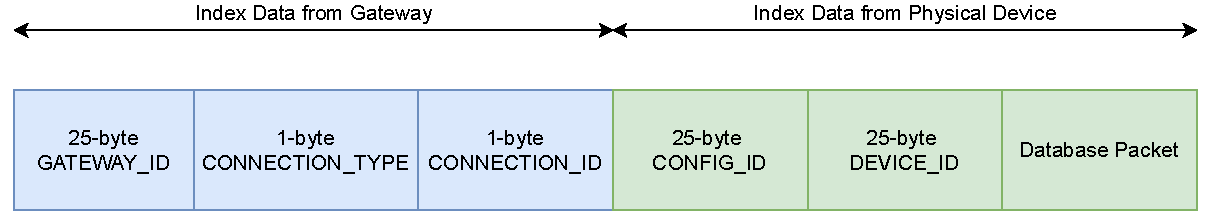
\includegraphics[width=1.0\linewidth]{images/Thesis-Page-12-Hardware-data-frame-struct.pdf}
\caption{Cấu trúc gói dữ liệu trên frame giao tiếp với phần cứng.}
\label{fig:Hardware-data-frame-struct}
\end{figure}

\subsubsection{Giao tiếp với giao diện web}

\acrshort{api} server đóng vai trò như một \acrfull{rest} \acrshort{api} và Websocket server trong giao tiếp với giao diện web.

Trong vai trò \acrshort{rest} \acrshort{api} server, ứng dụng server cung cấp các dịch vụ tương tác với database theo cấu trúc \acrfull{crud} và phong cách \acrshort{rest} (minh họa như bảng \ref{tab:CRUD-REST-service}). Dựa trên cấu trúc này, giao diện web có thể truy xuất database thông qua các phương thức \acrshort{http} với cấu trúc \acrshort{crud} tương ứng. Hiện tại, giao diện web có thể truy xuất tới 5 \acrshort{rest} \acrshort{api}. Đó là:

\begin{itemize}
    \item ``config'': dịch vụ truy xuất dữ liệu các cấu hình chung cho tất cả thiết bị phần cứng.
    \item ``device'': dịch vụ truy xuất dữ liệu của một thiết bị vật lý cụ thể.
    \item ``UI'': dịch vụ truy xuất dữ liệu của một UI dashboard linh hoạt.
    \item ``user'': dịch vụ truy xuất dữ liệu của một người dùng.
    \item ``vStorage'': dịch vụ truy xuất dữ liệu của một \acrshort{vs}.
\end{itemize}

\begin{table}[htp]
\caption{Cấu trúc CRUD theo phong cách REST. Nguồn từ Wikipedia~\cite{CRUD-REST-Service}.}

\label{tab:CRUD-REST-service}%
\begin{center}
\begin{tabular}{|l|l|}
\hline
\textbf{CRUD} & \textbf{HTTP} \\ \hline
Create        & POST, PUT     \\ \hline
Read          & GET           \\ \hline
Update        & PUT, PATCH    \\ \hline
Delete        & DELETE        \\ \hline
\end{tabular}
\end{center}
\end{table}

Trong vai trò Websocket server, \acrshort{api} server đồng bộ (đề cập ở mục \ref{VSync-Mecha}) các sự thay đổi dữ liệu database với giao diện web. Cụ thể, dựa trên sự kiện ``change streams'' của MongoDB, dữ liệu của các \acrshort{vs} sẽ luôn được thông báo tới giao diện web. Cấu trúc dữ liệu gửi tới giao diện web là kiểu dữ liệu \acrfull{json} (minh họa như hình \ref{fig:VSSync-JSON-model}). Trong đó:

\begin{itemize}
    \item Trường ``cmd'' là lệnh yêu cầu đồng bộ dự liệu \acrshort{vs}.
    \item Trường ``data'' là trường dữ liệu cần đồng bộ. Trường này chứa ID của \acrshort{vs} (\textbf{\_vs\_id}), device ID (\textbf{dev\_id}), dữ liệu đồng bộ (\textbf{data}), và toàn bộ thuộc tính của \acrshort{vs} (\textbf{fullDocument}).
\end{itemize}

\begin{figure}[htp]
\centering
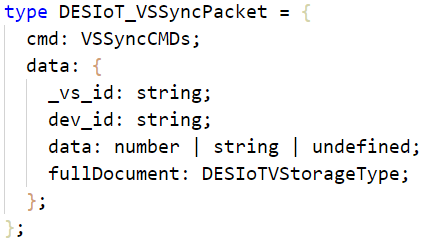
\includegraphics[width=0.5\linewidth]{images/fig-Hardware-data-frame-struct.png}
\caption{Cấu trúc dữ liệu JSON đồng bộ với giao diện web.}
\label{fig:VSSync-JSON-model}
\end{figure}

\subsubsection{Giao tiếp với database}

\acrshort{api} server tạo kết nối với MongoDB thông qua thư viện MongooseJS. Cụ thể, ứng dụng server kết nối với MongoDB qua phương thức \textbf{mongoose.connect()}. Cuối cùng, mongoose cung cấp giải pháp đơn giản, dựa trên schema để lập mô hình (model) dữ liệu trên ứng dụng server \cite{Mongoose-Solution}. Các model trong giao tiếp này bao gồm:

\begin{itemize}
    \item ``config'': cấu trúc document của các cấu hình chung cho tất cả thiết bị phần cứng.
    \item ``device'': cấu trúc document của một thiết bị vật lý cụ thể.
    \item ``UI'': cấu trúc document của một UI dashboard linh hoạt.
    \item ``user'': cấu trúc document của một người dùng.
    \item ``vStorage'': cấu trúc document của một \acrshort{vs}.
\end{itemize}

\subsection{MongoDB}

MongoDB là một hệ quản trị cơ sở dữ liệu miễn phí và mã nguồn mở đa nền tảng. Được phân loại như một hệ quản trị cơ sở dữ liệu NoSQL, MongoDB sử dụng các \acrshort{json}-like document với schema~\cite{MongoDB-Def}. Trên \acrshort{vps}, MongoDB hoạt động như một ứng dụng server. Cụ thể, ứng này được cài đặt bằng ``mongo Docker Image'' trên \textbf{docker-compose} và hoạt động trên cùng một \acrshort{vlan} với \acrshort{api} server và \acrshort{mqtt} Broker.

% connect and change streams
MongoDB thiết lập kết nối với \acrshort{api} server thông qua thư viện ``MongooseJS'' và cung cấp giải pháp cho việc đồng bộ với phần cứng và giao diện web. Cụ thể, MongoDB cung cấp giải pháp đồng bộ thông qua sự kiện ``change streams''. Sự kiện này giúp ứng dụng server theo dõi các thay đổi dữ liệu thời gian thực một cách dễ dàng. ``Change streams'' hoạt động trên ``Replica set'' của MongoDB.

% Replica set
Trên \acrshort{vps}, Mongo được triển khai trên mô hình ``Replica set''. Một \textit{replica set} trong MongoDB là một tập hợp các \textit{mongod} process mà duy trì cùng một data set. \textit{Replica set} cung cấp tính dự phòng (redundancy) và có sẵn cao (high availability), và là cơ sở cho tất cả quá trình phát triển sản phẩm~\cite{Mongo-Replication-Def}. Trên \acrshort{vps}, mô hình MongoDB \textit{Replica set} (minh họa như hình \ref{fig:MongoDB-Replication-Model}) bao gồm một \textit{primary} node và hai \textit{secondary} node.

\begin{figure}[htp]
\centering
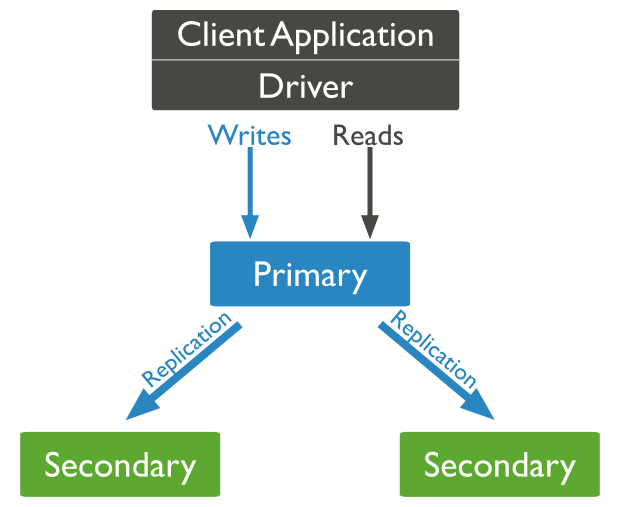
\includegraphics[width=0.7\linewidth]{images/replica-set-read-write-operations-primary.bakedsvg.png}
\caption{Mô hình MongoDB Replica Set trên VPS. Nguồn từ MongoDB~\cite{Mongo-Replication-Def}.}
\label{fig:MongoDB-Replication-Model}
\end{figure}

\section{Giao diện web}

%  Tổng quan
Giao diện web được xây dựng trên nền tảng Ant Design Pro, framework ReactJS, và ngôn ngữ TypeScript. Dựa trên nền tảng này, giao diện web sẽ được phát triển để cung cấp tương tác cho các admin dựa trên thư viện Ant Design và framework UmiJS.
% Những thành phần chính trên giao diện
Trên nền tảng Ant Design Pro, giao diện được trang bị sẵn Main Page (minh họa như hình \ref{fig:adp-default-mainpage}) và Login Page \ref{fig:adp-default-loginpage}). Main Page Layout bao gồm Page Header, Menu, Menu Header, Right Content, và Page Content; và Login Page cung cấp form để đăng nhập.

\begin{figure}[htp]
\centering
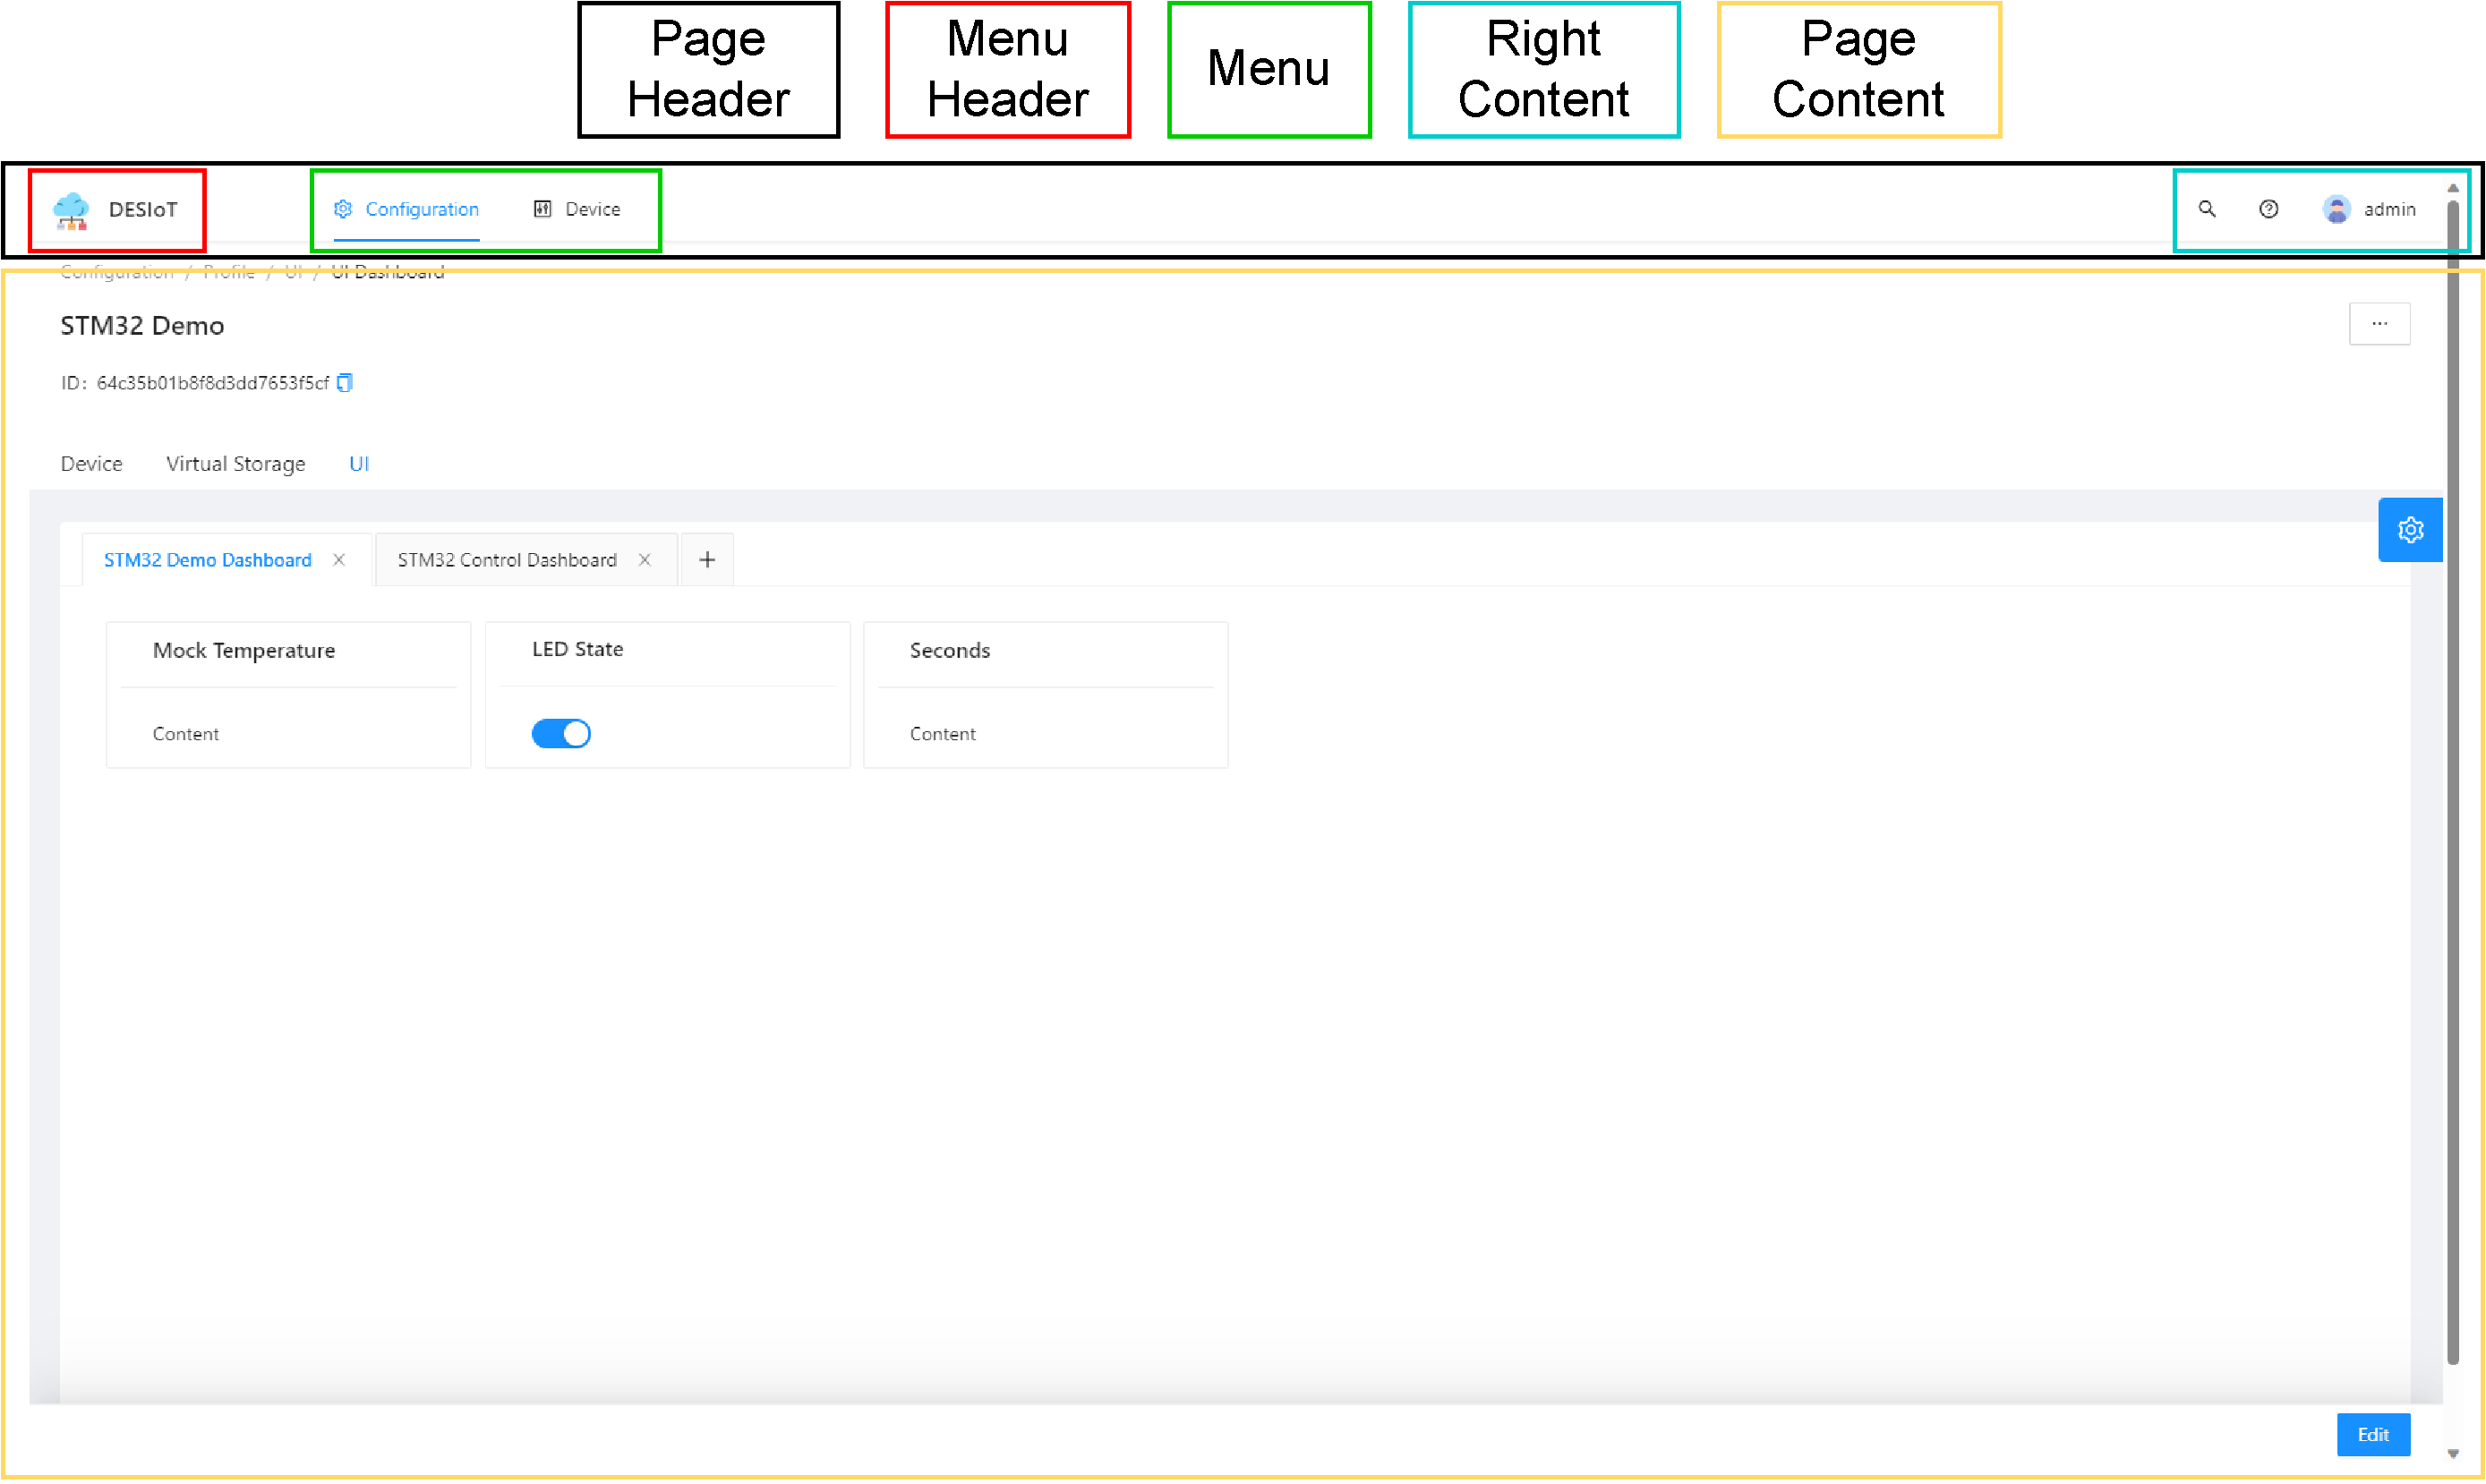
\includegraphics[width=1.0\linewidth]{images/Thesis-Page-13-adp-default-mainpage.pdf}
\caption{Layout của Main Page trên nền tảng Ant Design Pro.}
\label{fig:adp-default-mainpage}
\end{figure}

\begin{figure}[htp]
\centering
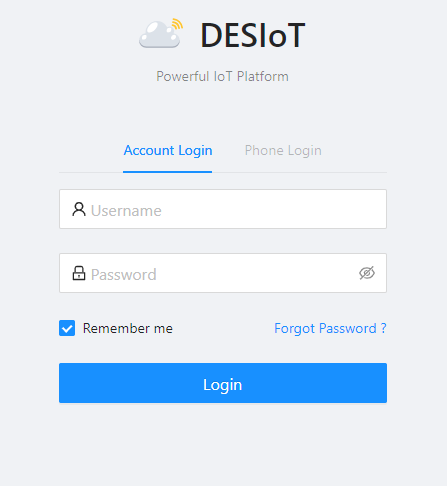
\includegraphics[width=0.7\linewidth]{images/fig-adp-default-loginpage.png}
\caption{Login Page trên nền tảng Ant Design Pro.}
\label{fig:adp-default-loginpage}
\end{figure}

% Các tương tác thiết lập trên giao diện web
Dựa trên nền tảng Ant Design Pro, giao diện web thiết lập các tương tác cho các quản trị viên. Các tương tác này chủ yếu diễn ra trên hai trang Configuration và Device.

\subsection{Configuration Page}

Configuration Page (minh họa như hình \ref{fig:config-page})hiển thị và cung cấp tương tác cho các cấu hình trên thiết bị phần cứng. Cụ thể, trên trang này, người dùng có thể quan sát, tạo mới, và truy cập một configuration.

\begin{figure}[htp]
\centering
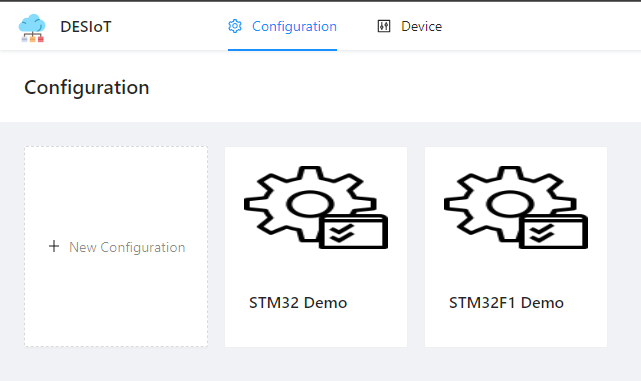
\includegraphics[width=0.7\linewidth]{images/fig-config-page.png}
\caption{Giao diện của Configuration Page.}
\label{fig:config-page}
\end{figure}

% Các tab
Khi mở một trang của một Configuration, người dùng có thể xem thông tin của Configuration. Ngoài ra, Configuration Page còn cung cấp các tab Device, Virtual Storage, và UI. Các tab này giúp truy xuất cơ sở dữ liệu trên model của một thiết bị phần cứng, \acrshort{vs}, và UI dashboard.

Trên tab Device, Device Tab (minh họa như hình \ref{fig:config-device-tab}) hiển thị danh sách thiết bị và người dùng có thể tạo mới hoặc xóa dữ liệu của một thiết bị thông qua \textbf{Add device} hoặc \textbf{Delete} button tương ứng. Dữ liệu của một device bao gồm ``Name'' và ``ID''.

\begin{figure}[htp]
\centering
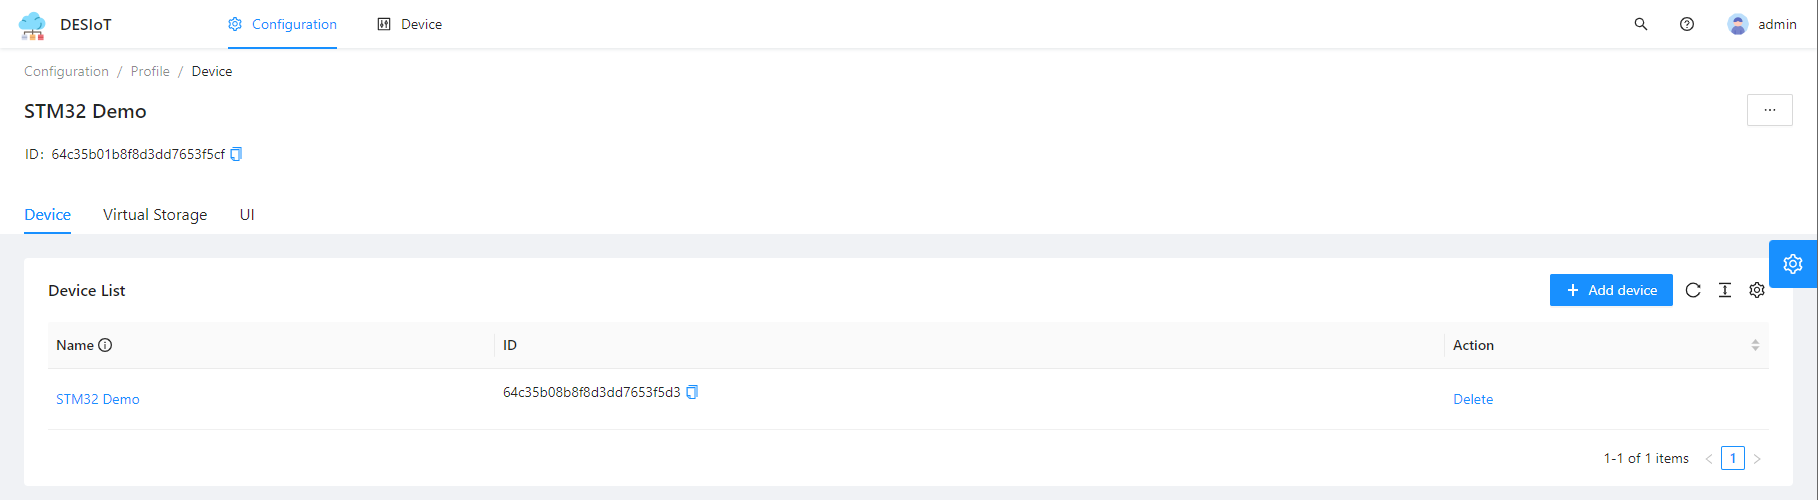
\includegraphics[width=1.0\linewidth]{images/fig-config-device-tab.png}
\caption{Giao diện của Device Tab trên Configuration Page.}
\label{fig:config-device-tab}
\end{figure}

Trên tab Virtual Storage, Virtual Storage Tab (minh họa như hình \ref{fig:config-vstorage-tab}) hiển thị danh sách các \acrshort{vs} và người dùng có thể tạo mới hoặc xóa dữ liệu của một \acrshort{vs} thông qua \textbf{Add Virtual Storage} hoặc \textbf{Delete} button tương ứng. Dữ liệu của một \acrshort{vs} bao gồm ``Name'', ``VStorage ID'', và ``Data Type''.

\begin{figure}[htp]
\centering
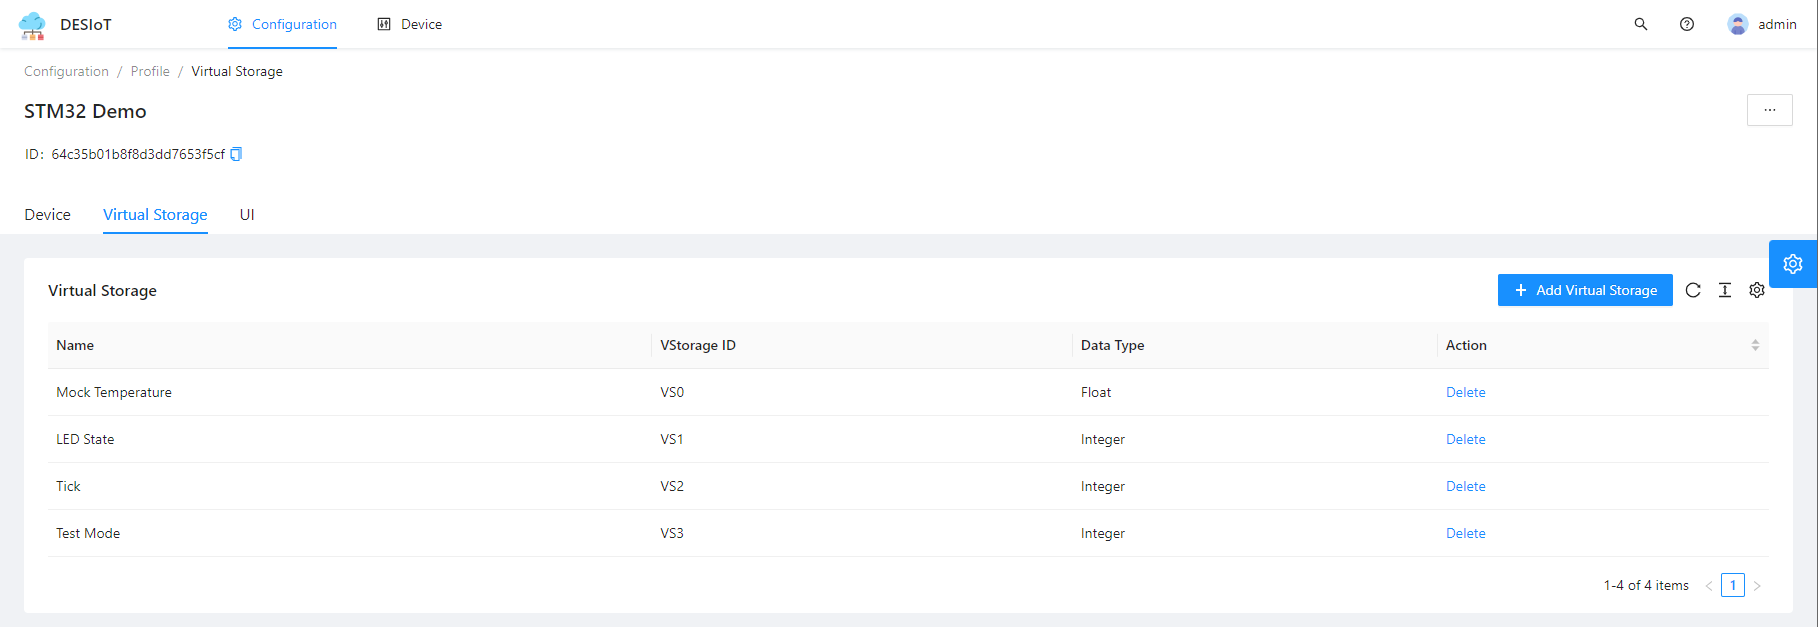
\includegraphics[width=1.0\linewidth]{images/fig-config-vstorage-tab.png}
\caption{Giao diện của Virtual Storage Tab trên Configuration Page.}
\label{fig:config-vstorage-tab}
\end{figure}

Trên tab UI, UI Tab (minh họa như hình \ref{fig:config-ui-tab}) hiển thị danh sách các Dashboard tab và người dùng có thể tạo mới hoặc xóa dữ liệu của một Dashboard thông qua ``+'' hoặc ``X'' button tương ứng. Trên mỗi Dashboard, người dùng có thể bật chế độ chỉnh sửa (minh họa như hình \ref{fig:config-ui-tab-edit-mode}) thông qua \textbf{Edit} button. Trên chế độ này, người dùng có thể thêm, xóa, hoặc chỉnh sửa các widget có sẵn để thiết kế Dashboard.

\begin{figure}[htp]
\centering
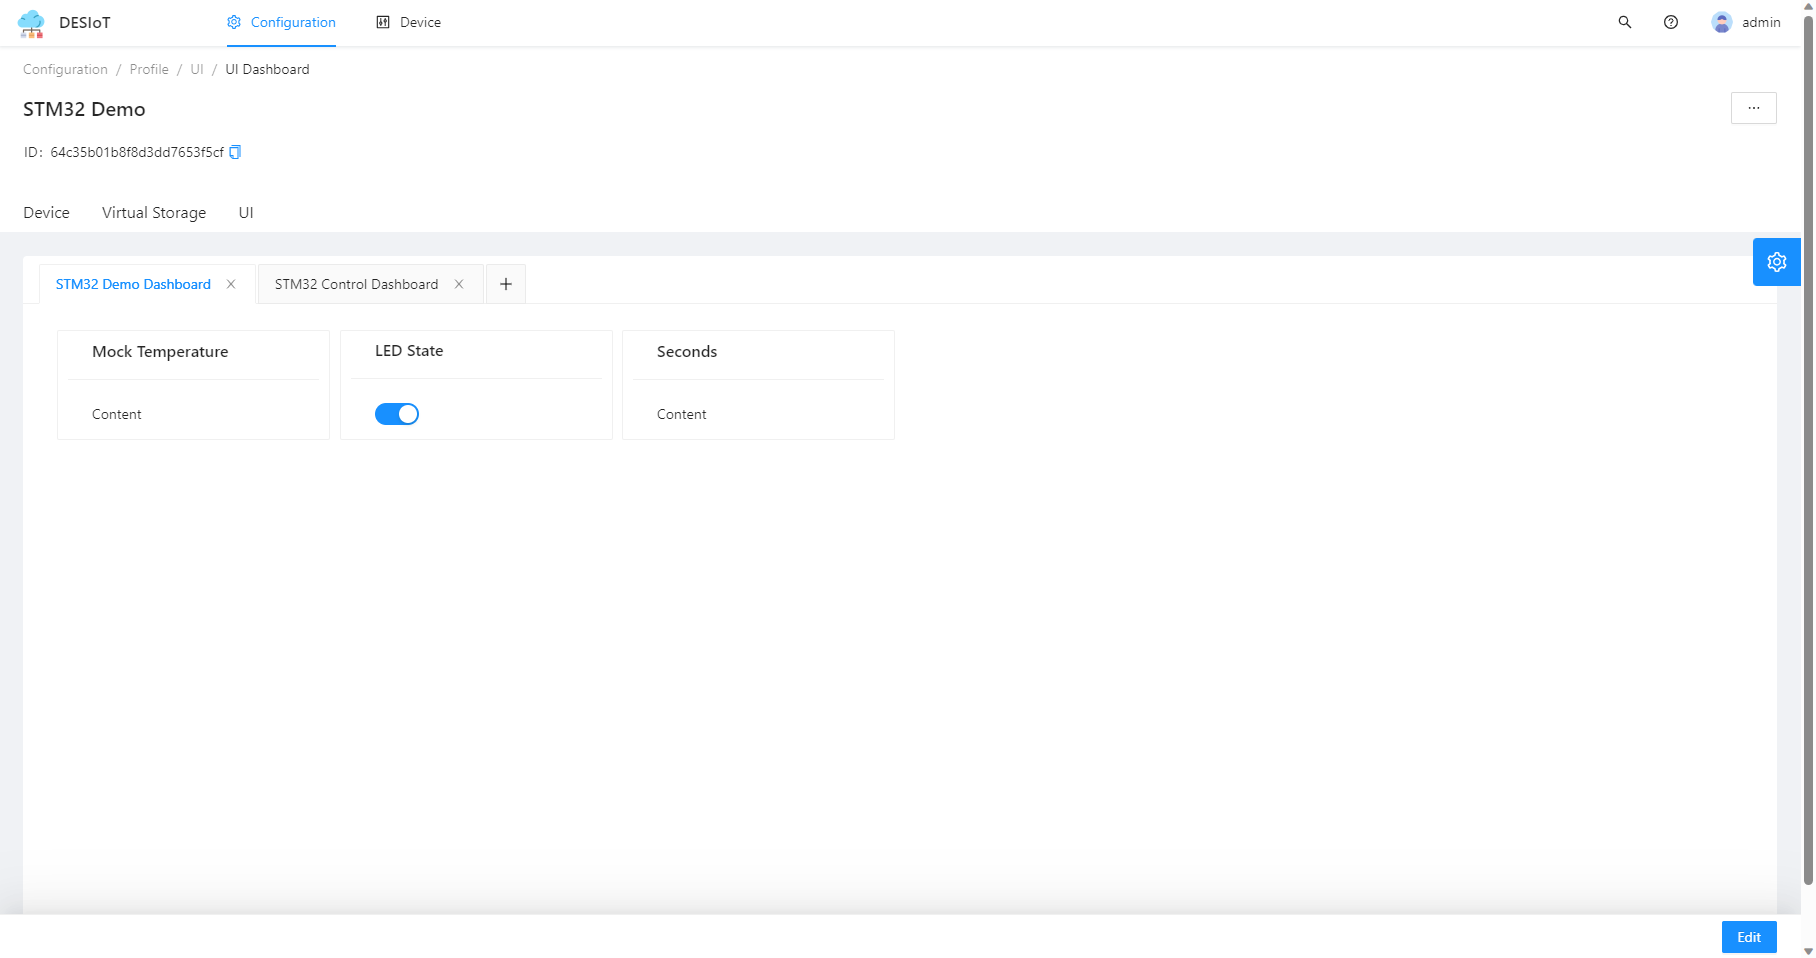
\includegraphics[width=1.0\linewidth]{images/fig-config-ui-tab.png}
\caption{Giao diện của UI Tab trên Configuration Page.}
\label{fig:config-ui-tab}
\end{figure}

\begin{figure}[htp]
\centering
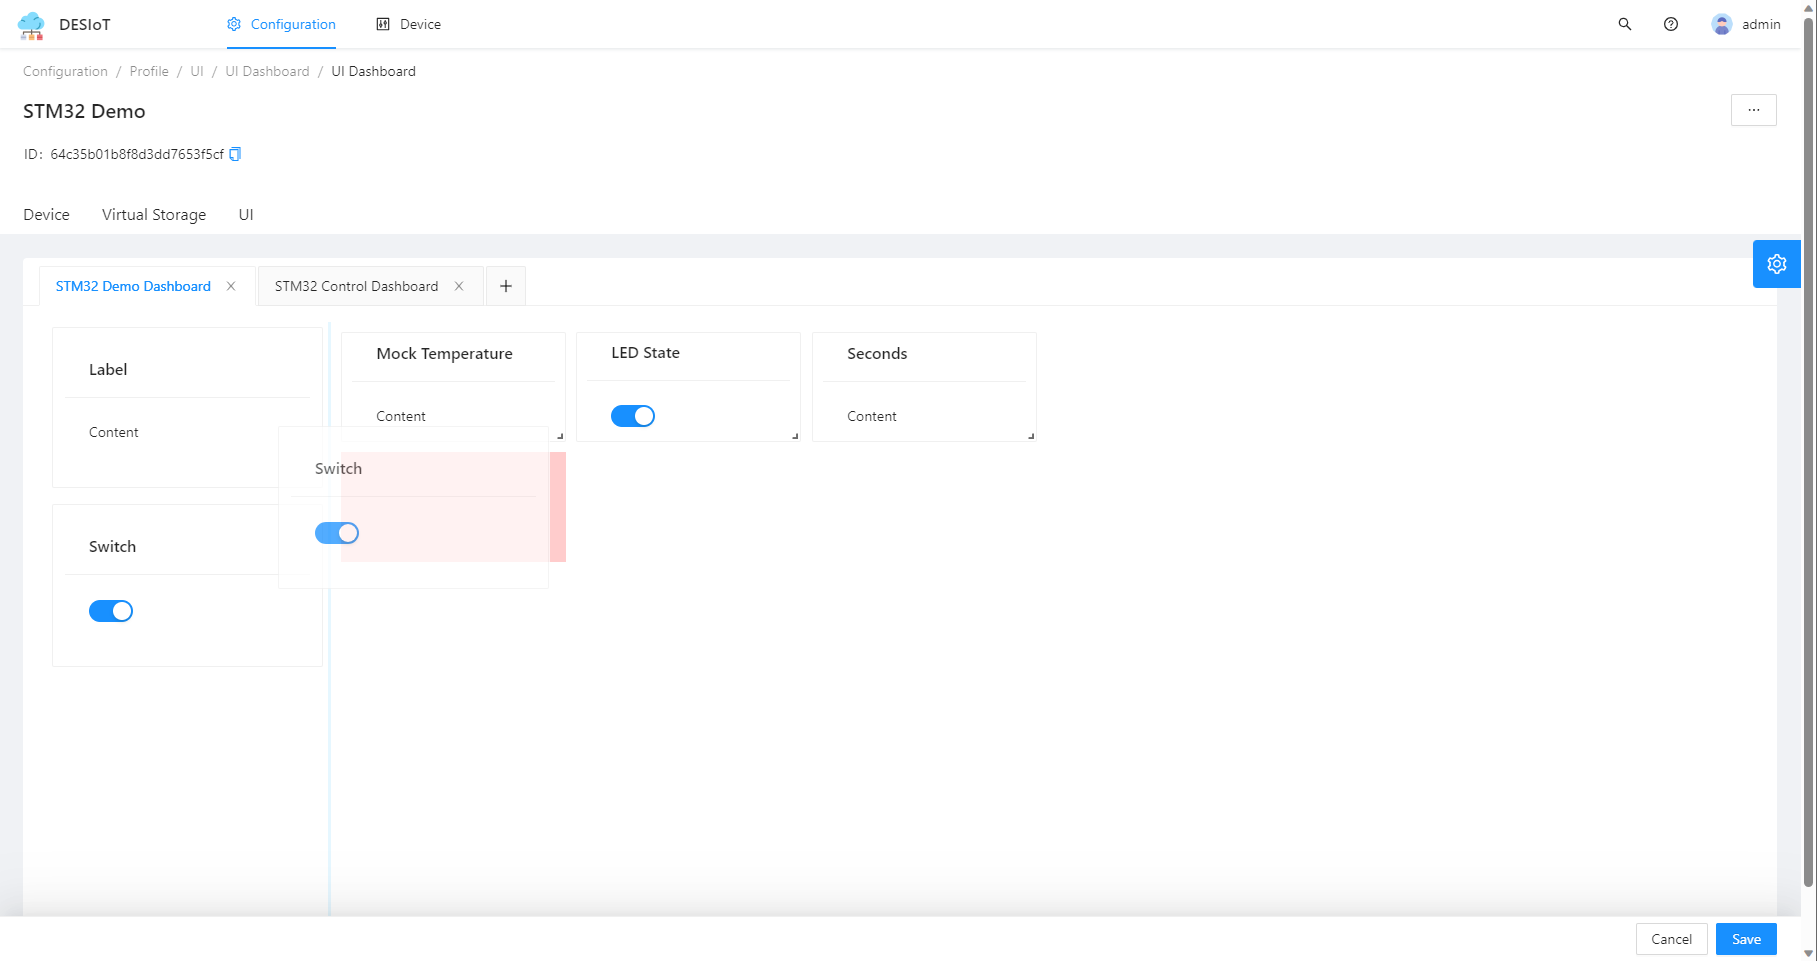
\includegraphics[width=1.0\linewidth]{images/fig-config-ui-tab-edit-mode.png}
\caption{Giao diện của UI Tab chế độ Edit trên Configuration Page.}
\label{fig:config-ui-tab-edit-mode}
\end{figure}

\subsection{Device Page}

Device Page (minh họa như hình \ref{fig:device-page}) hiển thị danh sách các thiết bị đã cấu hình trên Configuration Page. Khi mở một Device Tab, người dùng có thể lựa chọn UI Dashboard đã tạo và quan sát dữ liệu thời gian thực và điều khiển thiết bị trên dashboard.

\begin{figure}[htp]
\centering
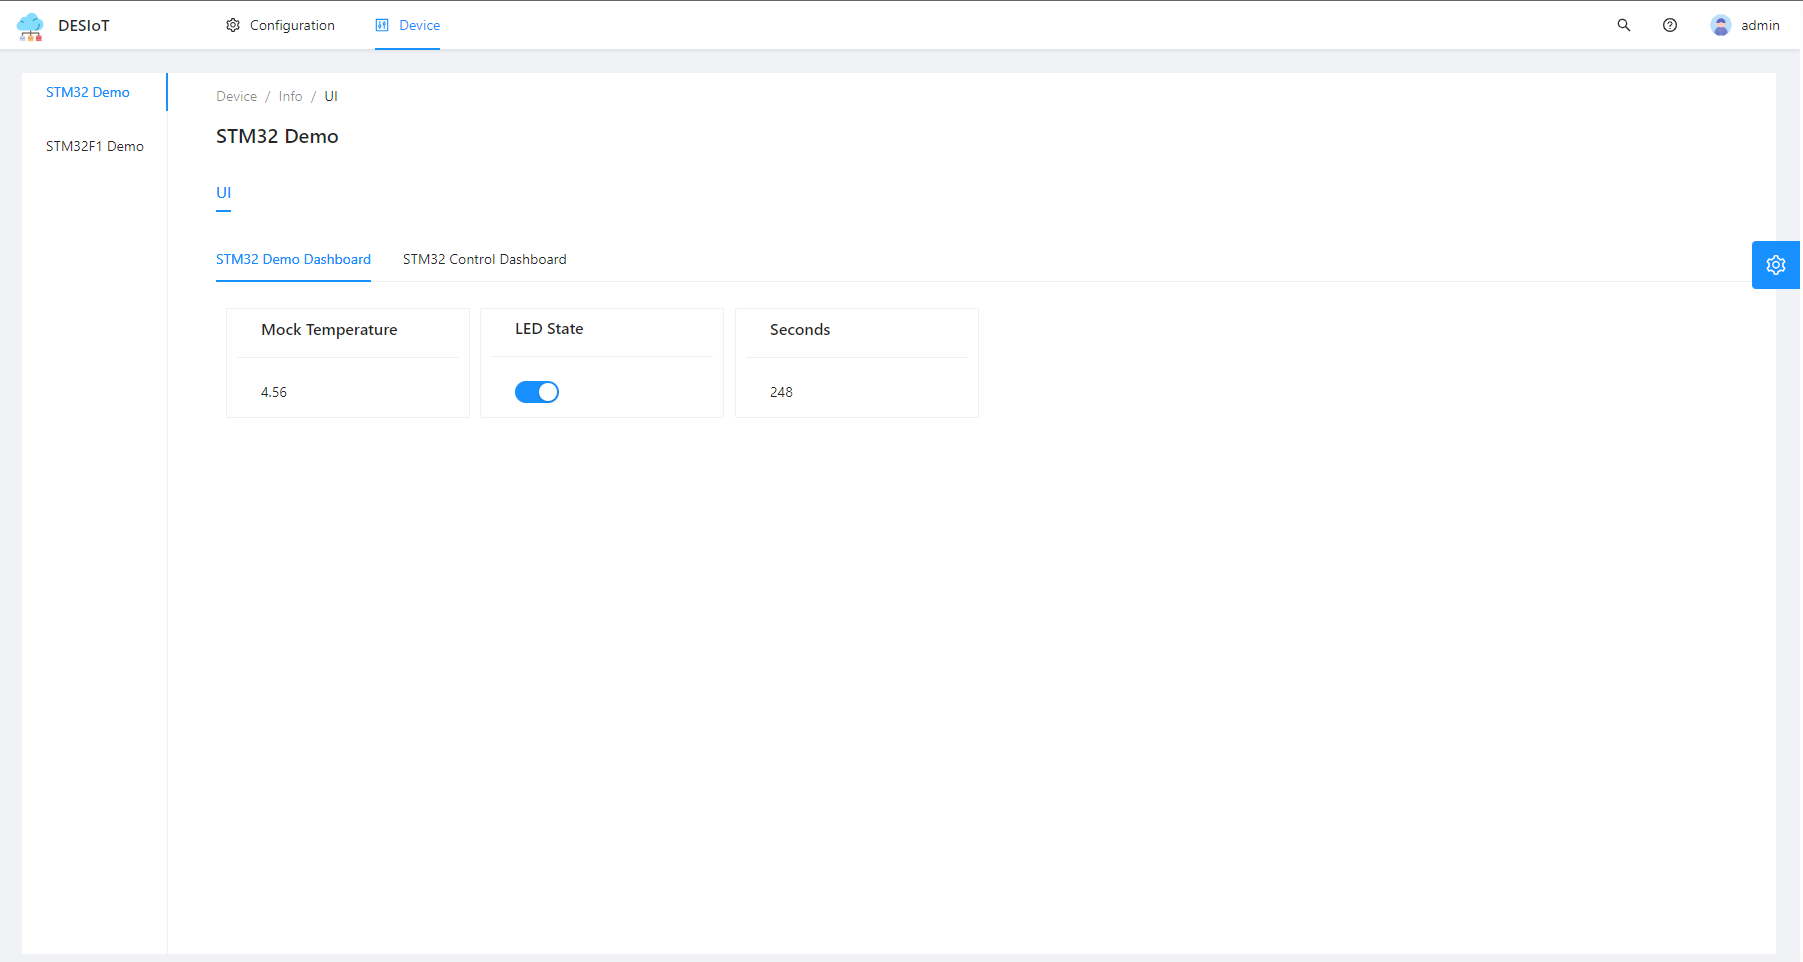
\includegraphics[width=1.0\linewidth]{images/fig-device-page.png}
\caption{Giao diện của Device Page.}
\label{fig:device-page}
\end{figure}